%%%%%%%% ICML 2025 ARTICLE DRAFT %%%%%%%%%%%%%%%%%%%%%%%%%%%%%%%%%
% Scope: the overall project and proposed framework; preliminary calibration results only.
% The bibliography is embedded so this is the only manuscript source to edit.
% Compile with the accompanying official ICML 2025 style files.
\begin{filecontents*}{article-references.bib}
@article{lindsey2026,
  author = {Lindsey, Jack},
  title = {Emergent Introspective Awareness in Large Language Models},
  journal = {arXiv preprint arXiv:2601.01828},
  year = {2026}, url = {https://arxiv.org/abs/2601.01828}
}
@article{hahami2026,
  author = {Hahami, Ely and Sinha, Ishaan and Jain, Lavik and Kaplan, Josh and Hahami, Jon},
  title = {Detecting the Disturbance: A Nuanced View of Introspective Abilities in {LLMs}},
  journal = {arXiv preprint arXiv:2512.12411},
  year = {2026}, note = {Version 2},
  url = {https://arxiv.org/abs/2512.12411v2}
}
@article{macar2026,
  author = {Macar, Uzay and Yang, Li and Wang, Atticus and Wallich, Peter and Ameisen, Emmanuel and Lindsey, Jack},
  title = {Mechanisms of Introspective Awareness},
  journal = {arXiv preprint arXiv:2603.21396},
  year = {2026}, url = {https://arxiv.org/abs/2603.21396}
}
@article{fornasiere2026,
  author = {Fornasiere, Damiano and Bronzi, Mirko and Kitts, Spencer and Palmas, Alessandro and Bengio, Yoshua and Richardson, Oliver},
  title = {Language Models Recognize Dropout and {Gaussian} Noise Applied to Their Activations},
  journal = {arXiv preprint arXiv:2604.17465},
  year = {2026}, url = {https://arxiv.org/abs/2604.17465}
}
@article{singh2026,
  author = {Singh, Shashwat and Linzen, Tal and Ravfogel, Shauli},
  title = {Can {LLMs} Introspect? A Reality Check},
  journal = {arXiv preprint arXiv:2605.26242},
  year = {2026}, note = {Accepted at COLM 2026},
  url = {https://arxiv.org/abs/2605.26242}
}
@article{nguyen2026,
  author = {Nguyen, Tam and Nguyen, Tu Anh and Alemohammad, Sina and Baraniuk, Richard G.},
  title = {Minimizing Collateral Damage in Activation Steering},
  journal = {arXiv preprint arXiv:2605.01167},
  year = {2026}, url = {https://arxiv.org/abs/2605.01167}
}
@article{ferrara2026,
  author = {Ferrara, Emilio},
  title = {Open-Weight Masked Introspection: Measuring What Language Models Can Report About Their Own Computation},
  journal = {arXiv preprint arXiv:2608.20569},
  year = {2026}, url = {https://arxiv.org/abs/2608.20569}
}
@article{kowalski2026,
  author = {Kowalski, Marek Mateusz and {Fonseca Rivera}, Joshua and Macar, Uzay and Africa, David Demitri},
  title = {Measuring Activation Control in Large Language Models},
  journal = {arXiv preprint arXiv:2608.21664},
  year = {2026}, url = {https://arxiv.org/abs/2608.21664}
}
@article{fleming2014,
  author = {Fleming, Stephen M. and Lau, Hakwan C.},
  title = {How to Measure Metacognition},
  journal = {Frontiers in Human Neuroscience},
  volume = {8}, pages = {443}, year = {2014},
  doi = {10.3389/fnhum.2014.00443},
  url = {https://doi.org/10.3389/fnhum.2014.00443}
}
\end{filecontents*}

\documentclass{article}
\usepackage[T1]{fontenc}
\usepackage{microtype}
\usepackage{graphicx}
\usepackage{subfigure}
\usepackage{booktabs}
\usepackage{float}
\usepackage{hyperref}
\newcommand{\theHalgorithm}{\arabic{algorithm}}
\usepackage[accepted]{icml2025}
\usepackage{amsmath}
\usepackage{amssymb}
\usepackage{mathtools}
\usepackage{amsthm}
\usepackage[capitalize,noabbrev]{cleveref}

% Retain the supplied template's layout without claiming ICML publication.
\icmltitlerunning{Psychophysics of Internal Perturbation Detection in Language Models}
\makeatletter
\renewcommand{\Notice@String}{Research manuscript draft. ICML 2025 template.}
% Name only until the corresponding author's email is supplied.
% Replace this definition with \icmlcorrespondingauthor{Name}{email} later.
\newcommand{\icmlcorrespondingauthor@text}{Seif Zaafouri}
\makeatother

\begin{document}
\twocolumn[
\icmltitle{Psychophysics of Internal Perturbation Detection in Language Models:\\
            Introspection, Anomaly, or Geometry?}
\begin{icmlauthorlist}
\icmlauthor{William Auroux}{project}
\icmlauthor{Thomas Gegout}{project}
\icmlauthor{Louis Le Dain}{project}
\icmlauthor{Seif Zaafouri}{project}
\end{icmlauthorlist}
% Replace this project identifier with the authors' institutional affiliation.
\icmlaffiliation{project}{Sujet 15 research project, supervised by Fabrice Popineau}
\icmlkeywords{large language models, introspection, psychophysics, activation steering, metacognition}
\vskip 0.3in
]
\printAffiliationsAndNotice{}

\begin{abstract}
Language models can sometimes report changes to their internal activations, but it remains unclear whether these reports reflect sensitivity to conceptual content, generic anomaly detection, response bias, or disrupted computation.
We propose a computational psychophysics framework to distinguish these explanations within a common experimental setting.
Using Llama-3.1-8B-Instruct as the primary model, the framework compares conceptual interventions, fixed random directions, renewed noise, and dropout across depth and intensity, under both raw and naturally standardized dose matching.
It combines psychometric localization curves with presence judgments, sham trials, a semantic control task, and textual induction to separate sensitivity from response preference, task degradation, and input-driven reports.
Confidence judgments and extensions to multiple interventions address what information reports convey beyond a binary decision, including intervention number, content, and relative depth.
The objective is to characterize the conditions and limits of internal perturbation reporting through convergent behavioral measurements, without treating successful detection as sufficient evidence of introspection.
\end{abstract}

\section{Introduction}

Can a language model distinguish a change in its own computation from a change in what it reads?
This question matters for interpreting model self-reports and assessing their potential use in oversight.
Activation interventions make it experimentally tractable: a known perturbation is introduced into a model, and its subsequent report is compared with the intervention actually applied.
Existing studies reveal both successful reports and substantial dependence on task, model, depth, and response format \citep{lindsey2026,hahami2026,macar2026}.
The challenge is to determine what those successes measure.

Several explanations remain compatible with above-chance performance.
A model might recognize conceptual content, respond to a generic computational anomaly, or favor a response token whose score has shifted.
At sufficiently high intensity, a report might also accompany broad task disruption.
Conversely, a binary response can conceal information expressed in confidence or continuous output scores.
These alternatives cannot be resolved by a single detection accuracy or by comparing results obtained with different interventions and prompts.

Our project approaches this problem through computational psychophysics.
Its central question is whether differences in detectability between conceptual and nonconceptual perturbations persist when intensity is expressed in raw units or relative to natural activation variability.
Around this comparison, we test whether reports track intervention location and presence, whether sensitivity varies across concepts and layers, and whether detection remains measurable when semantic task performance is preserved.
Textual induction tests false reports without an internal intervention, while confidence and multiple-intervention tasks probe the specificity of the information available to the model.

The proposed contribution is a common framework connecting dose--response curves, response-bias controls, functional integrity, and report specificity.
It treats localization as a measurement instrument and distinguishes behavioral sensitivity from stronger claims about metacognitive monitoring.
We first situate this framework in the literature and describe its main hypotheses and comparisons; the subsequent experimental section separately presents the calibration study and its observed results.

\section{Related Work}

\paragraph{Reporting internal interventions.}
\citet{lindsey2026} introduced experiments in which models sometimes detect and identify injected conceptual representations, with substantial dependence on model and context.
\citet{hahami2026} showed that binary reports in Llama-3.1-8B-Instruct can be confounded by global shifts toward affirmative responses, while localization and relative-intensity judgments reveal differential sensitivity to early-layer interventions.
In other models and settings, \citet{macar2026} found detection that cannot be explained by a simple affirmative-response association and traced a circuit separating perturbation evidence from the default negative response.
These findings support careful distinctions between detection, identification, and response bias; their different tasks and intervention settings prevent a direct ranking of introspective ability.

\paragraph{Nonconceptual perturbations and interpretation.}
\citet{fornasiere2026} demonstrated localization of dropout and Gaussian noise in several model families, together with some ability to distinguish perturbation types.
Detection therefore need not depend on an injected semantic concept.
More broadly, \citet{singh2026} argue that evidence for introspection must require both privileged access to internal states and second-order computation.
Their controls show that input manipulations can elicit reports resembling those caused by internal interventions.
We accordingly treat perturbation detection as a behavioral discrimination problem, without equating successful discrimination with metacognitive monitoring.

\paragraph{Geometry and intervention strength.}
\citet{nguyen2026} model collateral effects of activation steering using the empirical second moment of activations, accounting for nonuniform costs across directions.
Their objective is to preserve unrelated capabilities, rather than measure perturbation detection, but it motivates attention to geometry when comparing interventions.
This makes intensity and task degradation joint concerns: matching displacement norms need not match either natural variability or functional impact.
Our framework combines dose comparisons with a separate semantic task to assess whether detectable perturbations preserve useful computation.

\paragraph{Information, confidence, and control.}
\citet{ferrara2026} found that intervention information can be decodable internally without useful discrimination by the discrete report; in one tested model, confidence nevertheless distinguishes intervention from sham.
This motivates measuring continuous evidence alongside categorical responses.
Following \citet{fleming2014}, we distinguish sensitivity to intervention presence from metacognitive sensitivity, which concerns whether confidence predicts decision correctness.
Separately, \citet{kowalski2026} show that models can modulate activations on instruction, a capability that should not be conflated with detecting an externally imposed change.
Together, these studies motivate measuring what a report contains---presence, location, content, or confidence---rather than treating different tasks as interchangeable measures of introspection.

\section{Proposed Approach}
\label{sec:proposal}

The framework organizes the project around three questions: what determines detectability, which alternative explanations survive behavioral controls, and how specific the reported information is.
The comparisons below constitute the proposed experimental program; their outcomes are not inferred from the calibration results reported later.

\subsection{Perturbation Type, Dose, and Depth}

The primary model is Llama-3.1-8B-Instruct.
The main design compares four intervention families at individual decoder-block outputs across all 32 layers: concept-derived directions, fixed isotropic random directions, noise whose direction is renewed per targeted token, and dropout.
Concept versus random contrasts address constructed semantic content, while fixed versus renewed directions address spatial coherence across tokens.
Dropout provides a qualitatively different, activation-dependent perturbation.

For additive interventions, $h'_{\ell,t}=h_{\ell,t}+\alpha v$ with $\|v\|_2=1$, so $\alpha$ is the displacement norm per targeted token.
Two distinct matching rules compare equal raw amplitudes and equal standardized doses,
\begin{equation}
 z=\frac{\alpha}{s(\ell,v)},
 \qquad \alpha=z\,s(\ell,v),
 \label{eq:dose}
\end{equation}
where $s(\ell,v)>0$ measures natural directional variability in the intended presentation context.
We estimate $s(\ell,v)$ before behavioral evaluation from unperturbed projections at the same activation site and eligible token positions used for intervention.
The sample standard deviation is the primary estimator, corrected median absolute deviation (MAD) provides a robust sensitivity analysis, and uncertainty is assessed by resampling sentences with their tokens kept together.
The initial development run covers 100 sentences, 616 token positions, all 32 decoder blocks, ten concept directions and ten fixed random directions per block, and one renewed-noise direction per position.

Two-alternative forced-choice localization supplies psychometric curves under both dose rules.
Counterbalancing sentence order and intervention target tests whether preference follows the perturbed sentence rather than its label or position.
The primary hypotheses are that curves differ between families at matched raw amplitude and that standardization changes these contrasts.
Thresholds at 75\% correct summarize the curves where supported by the tested range; variation across concepts, random directions, and layers tests whether family averages conceal heterogeneous sensitivity.
Thresholds are not extrapolated when unobserved, and nonmonotonic behavior at high doses remains part of the result.

\subsection{Sensitivity and Alternative Explanations}

Presence judgments complement localization by including trials with no intervention.
Sham trials and reversed response mappings allow hit rates, false-positive rates, sensitivity $d'$, and response criterion to be distinguished.
This tests whether a model detects a real intervention beyond its tendency to declare one, a question that localization alone cannot answer.

A separate semantic classification task measures whether detection occurs while useful task performance is preserved.
Its queried concept differs from the injected concept, reducing direct answer steering.
In parallel, textual induction crosses concept-evoking versus weakly evocative text with injection versus sham.
This tests whether the input alone increases false declarations of internal intervention, without assuming that text and activation injection produce equivalent internal states.
Together, these controls address response bias, general disruption, and input-driven anomaly reports as competing explanations.

\subsection{Confidence and Report Specificity}

Ordinal confidence and response-logit margins test whether continuous scores contain information absent from a binary answer.
We distinguish discrimination of intervention presence from the relation between confidence and correctness, using type-2 measures and meta-$d'$ only when trial counts support estimation.
Such measures characterize reporting performance without establishing a second-order mechanism.

Extensions to multiple interventions ask whether the model can report their number, identify two injected concepts, and judge their relative order across layers.
Counting is compared under constant per-injection dose and constant aggregate standardized budget to separate event number from cumulative intensity.
Content and relative-depth judgments use counterbalanced concept assignments and matched doses.
These extensions probe whether reports preserve distinctions between internal events beyond a generic sense that something changed; the single-intervention comparisons remain the primary program.

Across the framework, a shared sentence corpus, recorded intervention sites, and matched comparisons support attribution of differences to the manipulated factors.
Dose grids are selected through a pilot and fixed before the main measurements; uncertainty must respect shared sentences and directions.
Calibration and protocol choices are therefore part of measurement design, while the hypotheses above require their own behavioral evidence.

\subsection{Multi-injection for model perturbation}
\label{sec:multi-injection-approach}

The single-intervention program above asks whether a report tracks the presence, location, or content of one perturbation.
A complementary question is whether reports remain informative when several concept-derived interventions are present at once: can the model recover their number, their identity, and their relative depth, rather than only whether something changed at all?

We extend the additive intervention of \cref{eq:dose} to $n$ simultaneous injections, $h'_{\ell,t}=h_{\ell,t}+\sum_{i=1}^{n}\alpha_i v_i$, each concept direction $v_i$ applied at its own layer $\ell_i$ and sustained through generation.
Three tasks probe this setting using Llama-3.1-8B-Instruct.
\emph{Counting} injects $k\in\{0,\dots,4\}$ concept directions at distinct layers and requires a single forced digit response, with $k{=}0$ serving as the true sham.
\emph{Identification} varies what is actually injected---one concept, two concepts, one concept plus a random direction, or nothing---and asks the model to name what was injected, scored both by forced choice among labeled candidates and by free response.
\emph{Relative-depth ordering} injects two concepts at two layers and asks which was injected at the shallower layer, presented as a randomized \texttt{A}/\texttt{B} choice so that label assignment is decorrelated from true depth.
A fourth family, \emph{modulators}, reuses the ordering task while sweeping layer distance, the dose ratio between the two injections, and the cosine similarity of the injected concept pair.
All tasks draw from a pool of ten concept directions (five simple, five complex) applied across all 32 decoder blocks, with a coherence filter excluding degenerate or non-answer generations before scoring.
For this program, $\alpha$ plays the role of the standardized dose $z$ in \cref{eq:dose} directly, without a natural-scale recalibration in the injection context; this is a scope choice distinct from the raw-versus-standardized comparison of \cref{sec:proposal}.

A discrete decision can hide a default-answer preference unrelated to the injection, so each task pairs its accuracy metric with a control that isolates the injection's own contribution.
A \emph{bias-adjusted logit contrast} compares the first-token logit for the true answer against the model's default (e.g.\ $\mathrm{logit}(k)-\mathrm{logit}(\text{``1''})$ for counting), read directly from the generation call so it is available even for incoherent trials.
For ordering, a \emph{paired-sham} control repeats each injected trial with zero injection on the same prompt, so that $\text{contrast}_{\text{injected}}-\text{contrast}_{\text{sham}}$ isolates the injection's effect from the prompt's own baseline preference.

\section{Results}
\label{sec:results}

\subsection{Directional Scales Variations Across Layers and Directions}
\label{sec:calibration}

Across the 20,352 layer--direction pairs, all estimated standard deviations are finite and positive.
The principal result is a strong dependence on both layer and direction family: as shown in \cref{tab:scales,fig:scales}, concept directions have larger median scales than isotropic controls, particularly in early and intermediate blocks.
The concept-to-fixed-random ratio is approximately 122 at block~1, 35 at block~16, and 3.7 at block~30.
Equal raw amplitudes therefore correspond to markedly different standardized doses in this reference setting.

\begin{table}[H]
\centering
\small
\begin{tabular}{rrrr}
\toprule
Block & Concept & Fixed & Noise \\
\midrule
0  & 1.19   & 0.033 & 0.039 \\
1  & 177.45 & 1.450 & 2.124 \\
16 & 51.69  & 1.464 & 2.322 \\
30 & 12.07  & 3.266 & 2.138 \\
31 & 4.40   & 0.862 & 0.902 \\
\bottomrule
\end{tabular}
\caption{Median directional SD at five representative decoder blocks. Fixed denotes fixed random directions; Noise denotes renewed noise.}
\label{tab:scales}
\end{table}

\begin{figure}[H]
\centering
\includegraphics[width=\columnwidth]{figures/experiment_0_scales_sd.png}
\caption{Natural directional scales across decoder blocks. Concept directions are shown individually; controls are summarized by their median, interquartile range, and 5th--95th percentiles.}
\label{fig:scales}
\end{figure}

Because all directions have unit norm, these differences reflect their orientation relative to activation covariance rather than vector length; they do not establish that the additional variance is semantic.
SD and MAD also diverge strongly in internal layers, while the sentence-bootstrap coefficient of variation of SD remains about 0.8\% at the median across families.
The observed dispersion is therefore reproducible under sentence resampling, but sensitive to how scale is defined.

These values remain provisional because the development run presents sentences in isolation and therefore includes sequence-initial positions that are absent from the intended behavioral prompt.
The large between-family ratios cannot yet be interpreted as context-independent geometry or expected differences in detectability.
They instead show why the behavioral comparison requires scales recomputed in the matched prompt context before the dose grids are frozen.

\input{sections/experiment1}

\subsection{Multi-injection highlights the model's biases}
\label{sec:multi-injection-results}

Across counting, identification, and ordering (\cref{sec:multi-injection-approach}), the dominant finding is a strong, content-independent default-answer bias, not tracking of injection count, identity, or relative depth.
\Cref{tab:multi-injection-summary} summarizes the headline statistics; full per-dose numbers and the modulator sweeps are in \cref{app:multi-injection}.

\paragraph{Counting.}
At the true sham ($k{=}0$), the model answered ``1'' in 100\% of trials across both dosing regimes and every tested $\alpha$, never once answering ``0''; the response distribution stays concentrated on ``0''/``1'' regardless of the true count (\cref{fig:e9-dist}).
A bias-adjusted digit-logit contrast, $\mathrm{logit}(k)-\mathrm{logit}(\text{``1''})$, rules out a decoding-only account: it is strongly and consistently \emph{negative} at every dose (\cref{fig:e9-logit})---the raw logits themselves prefer ``1'' over the true count ($-1.81$ pooled, $t=-34.7$, $p=1.8\times10^{-186}$, $n=1{,}280$).

\paragraph{Identification.}
Forced-choice exact match (both slots correct) is 0.0--1.2\% in every condition, including \texttt{single\_concept} where only one slot names a specific concept; free-response similarity to the truly injected concept clears threshold in 2.8--4.7\% of trials (\cref{fig:e10}).
The one clean positive control is the sham condition's false-identification rate, exactly 0\%.

\paragraph{Relative-depth ordering.}
Raw accuracy is 53.0\%, not distinguishable from chance ($p=0.25$), and decomposes into a strong response-position bias: 94.9\% accuracy when the correct concept happened to be labeled \texttt{A}, 11.2\% when labeled \texttt{B}.
A bias-adjusted logit contrast initially suggested a small residual signal (mean $+0.38$ at $\alpha{=}2\text{--}3$, $t=1.28$, $p=0.20$), but the paired-sham control shows this was the prompt's own baseline preference: sham trials (zero injection, identical prompt) produce an almost identical contrast ($+0.258$) to injected trials ($+0.272$), leaving a double-adjusted, injection-specific contrast of $+0.014$ ($p=0.91$, $n=480$; \cref{fig:e11-sham}).

\paragraph{Modulators.}
Sweeping ordering against layer distance (E4) reproduces a positive, now nominally significant contrast ($+0.322$, $t=3.43$, $p=0.0006$, $n=1{,}680$) of the same sign and similar magnitude to ordering's own pre-sham result; given that result's fate above, E4 should be read as unconfirmed pending the same paired-sham test, not as established.
Dose ratio (E5) and concept similarity (E6) both show large apparent effects that fully decompose into the same \texttt{A}-bias once split by which letter was actually correct (\cref{fig:modulators-bias,app:multi-injection}), and E5's raw-accuracy trend is additionally confounded with dose magnitude exceeding the validated coherence range.

These results converge with the response-bias controls proposed in \cref{sec:proposal}: a discrete report can be dominated by a default answer that survives coherence filtering and, for counting, is present in the raw logits themselves---underscoring why localization and presence judgments alone cannot establish that a report tracks the manipulated factor.

\begin{table}[H]
\centering
\small
\begin{tabular}{lll}
\toprule
Experiment & Metric & Result \\
\midrule
Counting & $P(\text{``1''}\mid k{=}0)$ & 100\% \\
Counting & logit$(k)-$logit(``1'') & $-1.81$ \\
Identification & forced-choice exact match & 0.0--1.2\% \\
Ordering & raw accuracy & 53.0\% \\
Ordering & double-adj.\ contrast & $+0.014$ \\
\bottomrule
\end{tabular}
\caption{Headline null results across the multi-injection tasks. Full statistics, sample sizes, and $p$-values are given in the text and \cref{app:multi-injection}.}
\label{tab:multi-injection-summary}
\end{table}

\begin{figure}[H]
\centering
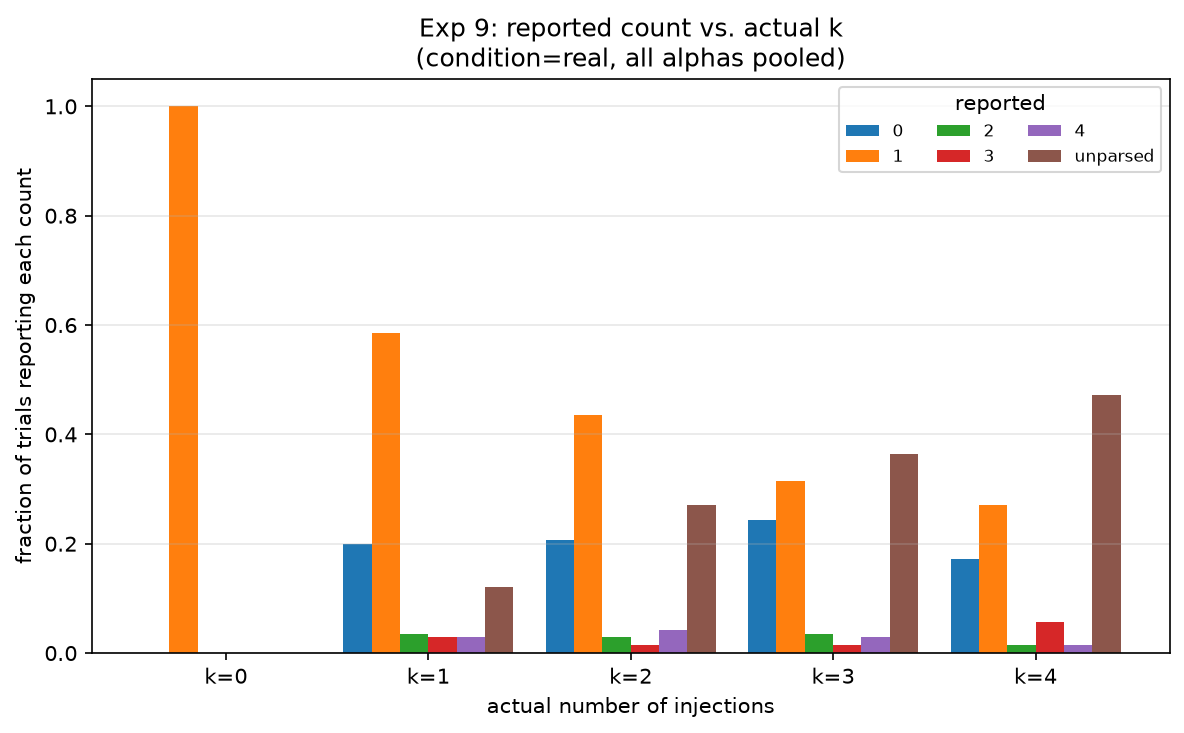
\includegraphics[width=\columnwidth]{figures/e9_response_distribution.png}
\caption{Reported count vs.\ true $k$: responses stay concentrated on ``0''/``1'' regardless of $k$.}
\label{fig:e9-dist}
\end{figure}

\begin{figure}[H]
\centering
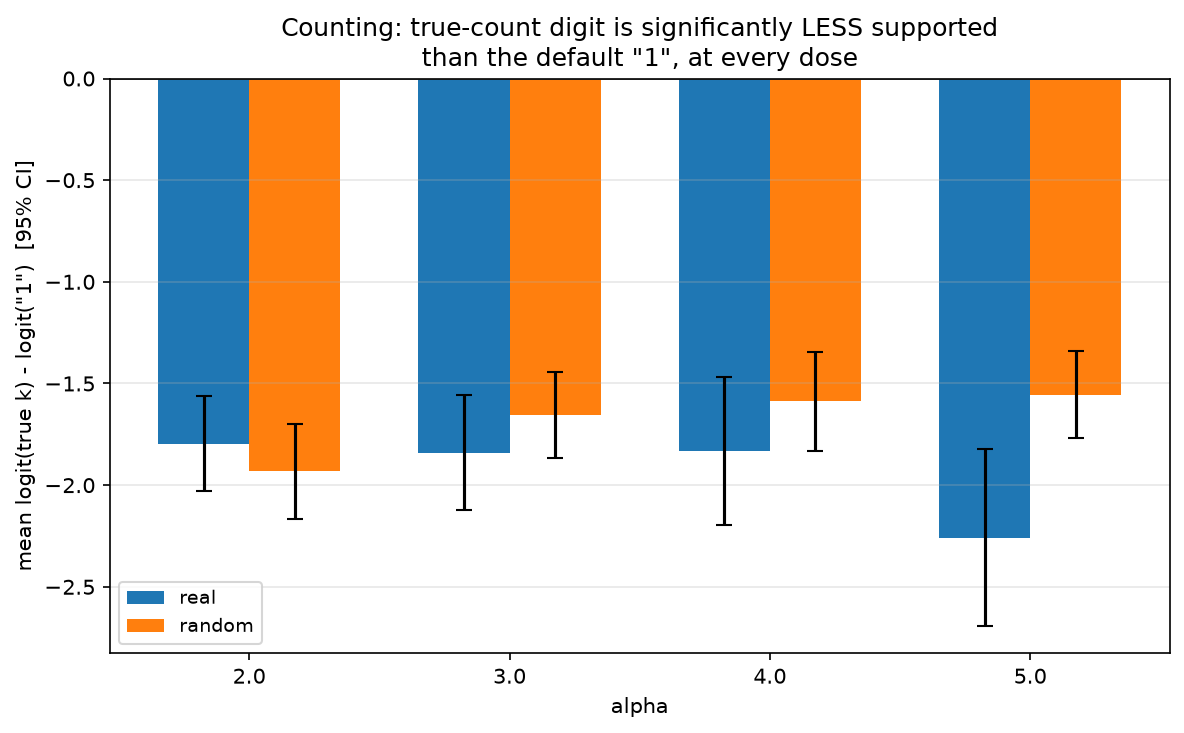
\includegraphics[width=\columnwidth]{figures/summary_counting_digit_logit_contrast.png}
\caption{Digit-level logit contrast $\mathrm{logit}(k)-\mathrm{logit}(\text{``1''})$, negative at every tested dose.}
\label{fig:e9-logit}
\end{figure}

\begin{figure}[H]
\centering
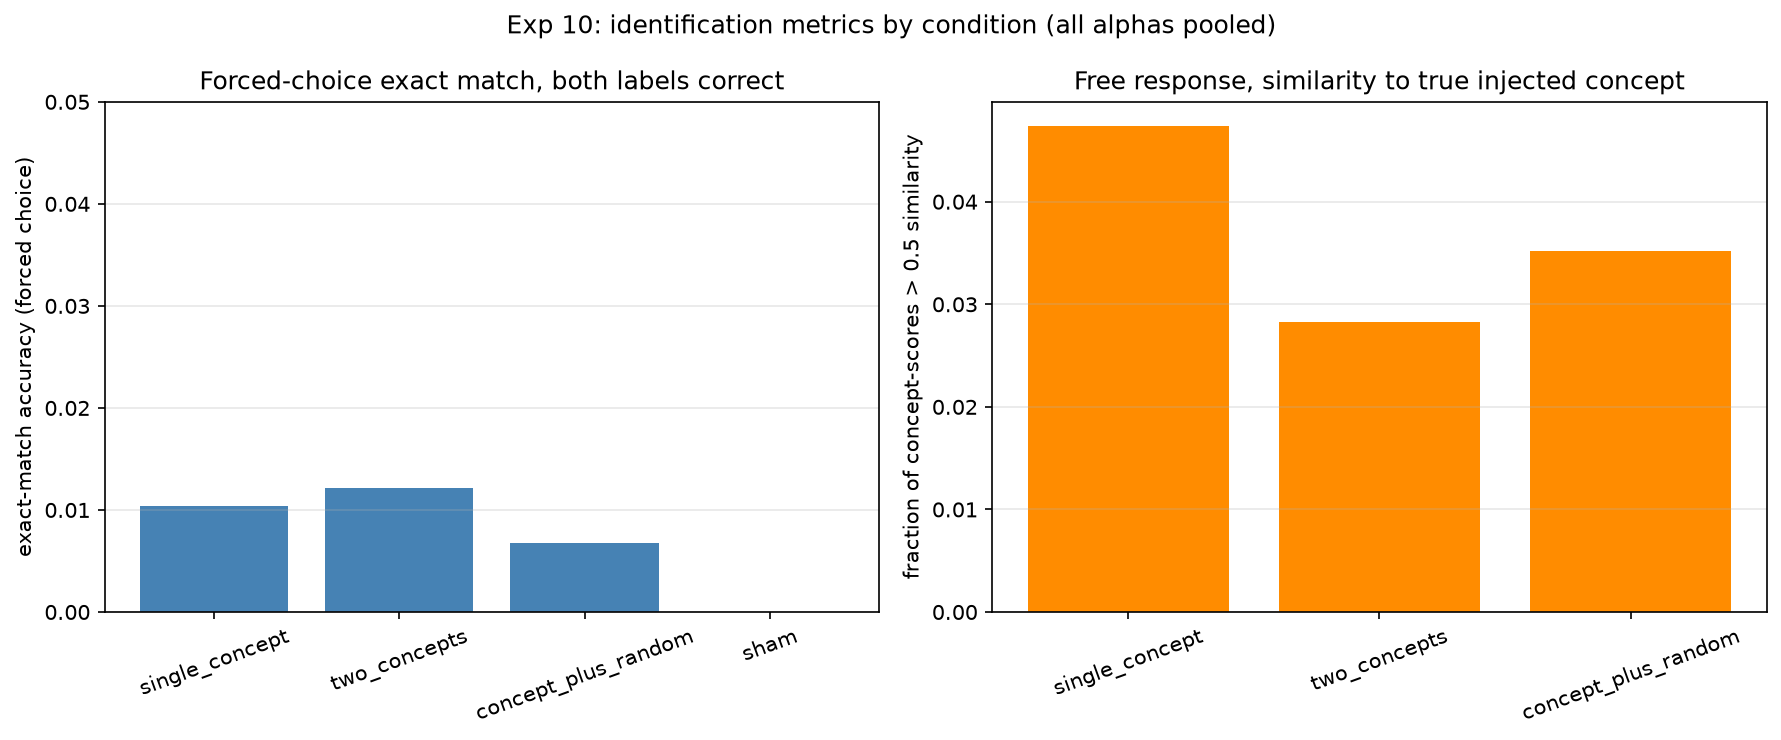
\includegraphics[width=\columnwidth]{figures/e10_metrics_by_condition.png}
\caption{Identification metrics by condition: forced-choice and free-response accuracy remain near floor throughout.}
\label{fig:e10}
\end{figure}

\begin{figure}[H]
\centering
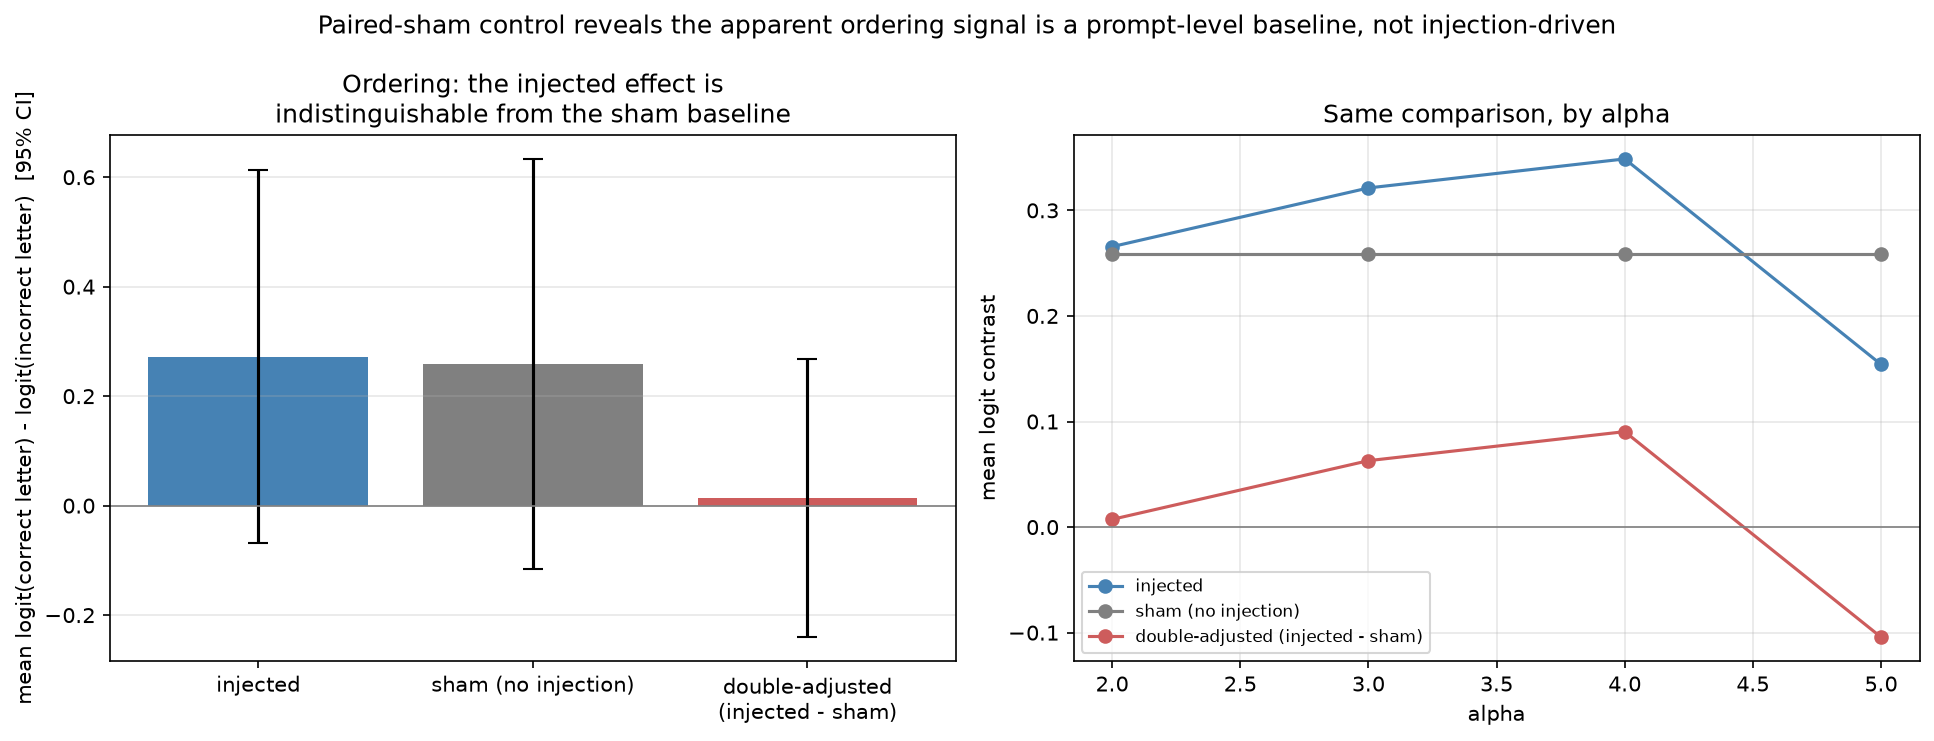
\includegraphics[width=\columnwidth]{figures/summary_ordering_sham_reveal.png}
\caption{Ordering: injected and paired-sham logit contrasts track each other closely; the double-adjusted, injection-specific contrast is flat around zero.}
\label{fig:e11-sham}
\end{figure}

\bibliography{article-references}
\bibliographystyle{icml2025}

\newpage
\onecolumn
\appendix
\section{Multi-Injection Experiments: Additional Details}
\label{app:multi-injection}

This appendix supplements \cref{sec:multi-injection-results} with the full experimental design, per-dose statistics, and the modulator bias decomposition referenced there.

\subsection{Design and trial counts}

\Cref{tab:multi-injection-trials} lists, for each task, the script, the manipulated conditions, and the number of trials collected in each of two experimental rounds.
Round 1 swept $\alpha\in\{1,\dots,7\}$ across all four tasks and is where the default-answer bias described in \cref{sec:multi-injection-results} was first observed.
Round 2 re-ran counting and ordering over a narrower $\alpha\in\{2,\dots,5\}$ range with the bias-adjusted logit contrast and, for ordering, the paired-sham control added; identification and the modulator sweeps were not re-run under Round 2 and so lack the sham control.

\begin{table}[h]
\centering
\small
\begin{tabular}{llrr}
\toprule
Task & Script & R1 trials & R2 trials \\
\midrule
Counting & \texttt{multi\_detection.py} & 5{,}600 & 2{,}880 \\
Identification & \texttt{multi\_identification.py} & 1{,}680 & --- \\
Ordering & \texttt{layer\_ordering.py} & 560 & 480 \\
Modulators (E4/E5/E6) & \texttt{modulators.py} & 2{,}940 & --- \\
\bottomrule
\end{tabular}
\caption{Trial counts per multi-injection task and round.}
\label{tab:multi-injection-trials}
\end{table}

\subsection{Per-dose statistics}

\Cref{tab:app-counting-dose} gives the counting digit-logit contrast by dose for the \texttt{individual} regime, real-injection condition; the \texttt{random}-direction condition tracks within about $0.2$ of these values at every dose.
\Cref{tab:app-ordering-dose} gives the ordering injected, sham, and double-adjusted contrasts by dose.
The sham contrast is essentially flat across dose, as expected for a condition with no injection, while the double-adjusted contrast stays within noise of zero at every tested $\alpha$, dipping slightly negative at $\alpha{=}5$.

\begin{table}[h]
\centering
\small
\begin{tabular}{rrr}
\toprule
$\alpha$ & Mean logit contrast & $n$ \\
\midrule
2 & $-1.80$ & 160 \\
3 & $-1.85$ & 160 \\
4 & $-1.83$ & 160 \\
5 & $-2.26$ & 160 \\
\bottomrule
\end{tabular}
\caption{Counting: digit-logit contrast by dose (individual regime, real condition).}
\label{tab:app-counting-dose}
\end{table}

\begin{table}[h]
\centering
\small
\begin{tabular}{rrrr}
\toprule
$\alpha$ & Injected & Sham & Double-adj. \\
\midrule
2 & $+0.266$ & $+0.258$ & $+0.007$ \\
3 & $+0.321$ & $+0.256$ & $+0.063$ \\
4 & $+0.349$ & $+0.259$ & $+0.090$ \\
5 & $+0.154$ & $+0.259$ & $-0.104$ \\
\bottomrule
\end{tabular}
\caption{Ordering: injected, sham, and double-adjusted logit contrast by dose ($n=120$ per row).}
\label{tab:app-ordering-dose}
\end{table}

\subsection{Modulators: a bias decomposition}

Taken at face value, the dose-ratio (E5) and concept-similarity (E6) sweeps both look strongly negative overall ($-0.574$, $p=3.5\times10^{-5}$ and $-0.874$, $p=2.9\times10^{-7}$ respectively).
Splitting by which letter was actually correct shows this is the same \texttt{A}-bias reported for ordering, not a ratio- or similarity-dependent effect: both sweeps show a strongly positive contrast when \texttt{A} happens to be the correct label and a strongly negative contrast when \texttt{B} does, and the negative overall average is an artifact of each sweep's random draw landing more \texttt{B}-correct trials than \texttt{A}-correct (E5: 336 vs.\ 224; E6: 441 vs.\ 259; \cref{fig:modulators-bias}).
E5's raw accuracy additionally drops sharply as the dose ratio grows, but this is confounded with dose magnitude: at ratio~8 and base $\alpha$ up to 7, the boosted injection's effective dose reaches 56, roughly eightfold outside the $\alpha$ range validated for coherent output.

\begin{figure}[h]
\centering
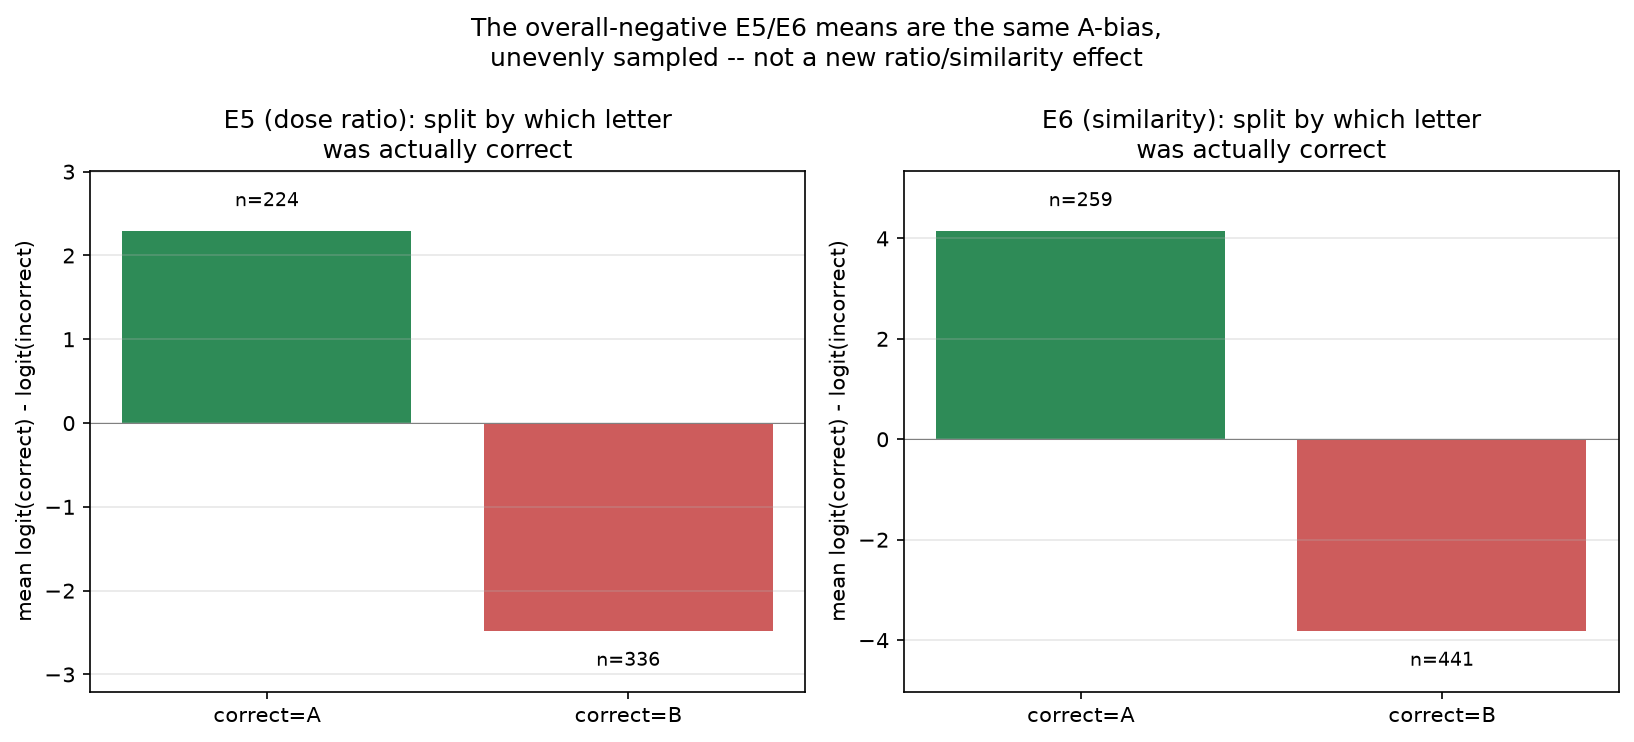
\includegraphics[width=0.7\columnwidth]{figures/modulators_e5_e6_bias_decomposition.png}
\caption{E5/E6 logit contrast split by which letter was actually correct: the large negative pooled averages are the same \texttt{A}-bias as elsewhere, not a ratio- or similarity-specific effect.}
\label{fig:modulators-bias}
\end{figure}

\subsection{Methodological notes}

Two implementation issues were identified and corrected during this program.
First, the coherence filter's default minimum-length threshold, tuned for open-ended calibration prompts, initially rejected valid single-character answers (e.g.\ ``1'', ``A'') under the strict single-token formats used here, silently corrupting downstream accuracy tables until corrected; all results above reflect the fix.
Second, the free-response grading model was moved to CPU after repeated GPU contention crashes when co-located with the 8B injection model on a shared node.

\subsection{Reproducibility}

Round 2 data are stored at \texttt{plots/multi\_detection\_trials\_\{individual,budget\}.pt} and \texttt{plots/layer\_ordering\_trials.pt}; Round 1 data are preserved separately for comparison.
Figures are generated by \texttt{reports/generate\_figures.py} and \texttt{reports/generate\_bias\_control\_figures.py}; per-dose breakdowns are reproduced by \texttt{code/analysis/count\_confusion\_matrix.py} and \texttt{code/analysis/ordering\_accuracy.py}.

\end{document}
